\documentclass[twocolumn,11pt]{article}
\setlength{\textheight}{9truein}
\setlength{\topmargin}{-0.9truein}
\setlength{\parindent}{0pt}
\setlength{\parskip}{10pt}
\setlength{\columnsep}{.4in}

\usepackage{amsmath,amsfonts,amssymb,amsthm,bm,caption,calc,ifthen,graphicx,url,hyperref}

\begin{document}
\pagestyle{plain}
\onecolumn
ASTP720 
\newline Homework 4
\newline Will Wainwright
\newline Repository: \href{https://github.com/wjwainwright/ASTP720}{https://github.com/wjwainwright/ASTP720}

\section*{Introduction}
Galaxy clusters are a collection of gravitationally bound galaxies. Despite the massive distances between these galaxies, over large, Gyr timescales we can expect to see these galaxies orbit and clump up. The Barnes-Hut algorithm is one way of determining the forces that a galaxy should experience that is computationally less expensive than the basic galaxy on galaxy force calculations. This method uses a data structure called trees, which is a tiered structure where nodes link to those above and below them. For certain applications, these trees can reduce the time it takes to access data and the subsequent computation time.

\section*{Methods}
The Barnes-Hut algorithm makes use of trees, which have nodes that behave like a tiered link list. To start, I created a class of galaxy objects that held parameters about their position and acceleration. The galaxy class also has a method to calculate the force on a given galaxy based on either other galaxies or the center of mass of a collective of galaxies within a given node, based on the criterion laid out in the notes. The acceleration calculation also employs force softening if the galaxies are close enough to each other. The acceleration calculation is used to update the positions of the galaxies for each step through the time series.

I then created a class of node objects that stored pointers to their parent node and any potential child nodes that they may be assigned. Nodes also have a set of coordinates to denote their positions, as they are synonymous with the boxes used in the Barnes-Hut algorithm. The node class has methods to add children and galaxies, to count the number of galaxies below a given branch of the tree, and to calculate the center of mass of a node.

I then created a tree class which is made up of a branching set of nodes. I initialize each tree with a token root node that does not store any galaxies but represents the bounding box for all of the subsequent nodes. The tree class has a method to add a galaxy to the tree, which recursively calls itself to traverse the tree and find where the galaxy belongs, splitting a leaf node into more nodes if the subdivisions are not adequate. The tree class also has a method to convert the tree into a linear list of nodes and two methods of plotting in either $XY$ or $XYZ$ coordinates.

A lot of the methods used to make the simulation possible, especially those that require traversal of the tree, are written recursively. Writing the methods in this way made sense for navigating the linked set of nodes, but is less intuitive to write and difficult to troubleshoot. For some methods, it made the most sense to store a list of galaxy pointers in the tree itself, as the structure of the tree did not benefit the computation time. I don't see this as an issue because the purpose of the tree structure is to aid in the calculation of forces across each time step.

The general process for using these methods starts with reading in the data from the given files. I initialize a tree with the starting positions of all 908 galaxies. The tree is built from the root, branching out only when two galaxies would otherwise occupy the same node. Once the tree is populated, I calculate the center of mass of every node in the tree. Then, for every time step until the desired end time is reached, I call the tree's evolve method. This method calculates the acceleration for every galaxy using the Barnes-Hut method, and then creates a new list of galaxies with positions that have been updated based on the acceleration over the given time step. The new list of galaxies is then fed into a new tree, and the evolve process is repeated.

\section*{Results}
I produced 3 major plots from the simulation, seen in Figures 1-3. I was unfortunately not able to do the extra steps on the homework past running the simulation, as I have already put $\sim$25 hours into the homework and wish to move on. My simulation takes about an hour and a half to run through the $10Gyr$ time series, but my assertion that all galaxies remain within the root node's bounding box is not met. If I let the simulation run with the error messages printing out every iteration, then I still get the results seen in Fig. 1 and Fig. 3. That being said, I'm not sure why a few of the galaxies are being flung outside of the simulation bounds even with force softening. It's possible that the time step is too large and therefore the force softening is not great enough, but without further testing I have to assume that it does not greatly affect the results of the simulation for the rest of the 900 odd galaxies.

Fig. 1 shows the path of three random galaxies throughout the $10Gyr$ time series. I can not vouch for the validity of the paths, but they seem to make sense given they are not being flung out into space or taking crazy jagged paths. I am not sure if the green path should be doing what appears to be a tight loop the loop, but who am I to question orbital mechanics. The comparison of the before and after pictures in Fig. 2 and Fig. 3 give me much more confidence that the simulation is working correctly, as we see the galaxies have a general trend of clumping together near the apparent center of mass. If the simulation were to run for $100Gyr$, I might expect to see a much more dense clump in the center, but also most likely far more galaxies flung into the deep depths as a result of inadequate force softening.

\begin{figure}[!h]
	\centering
	\noindent
	\makebox[\textwidth]{
      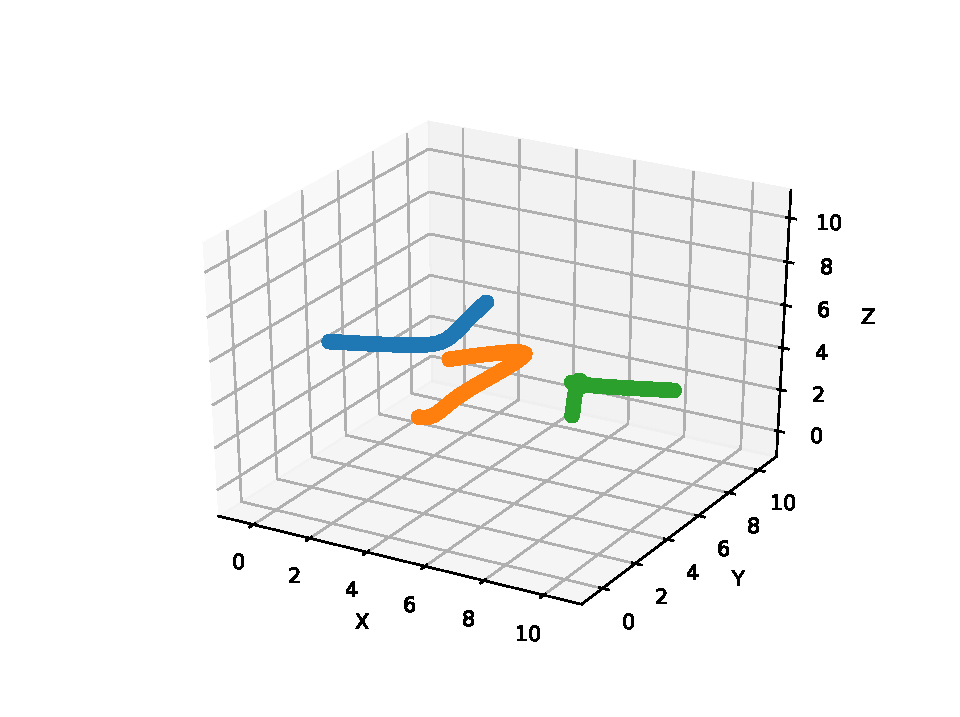
\includegraphics[width=4.5in]{10gyr.pdf}}
      \caption{3D plot of the positions of 3 galaxies through the cluster over the duration of the $10Gyr$ simulation.}
\end{figure}

\begin{figure}[!h]
	\centering
	\noindent
	\makebox[\textwidth]{
      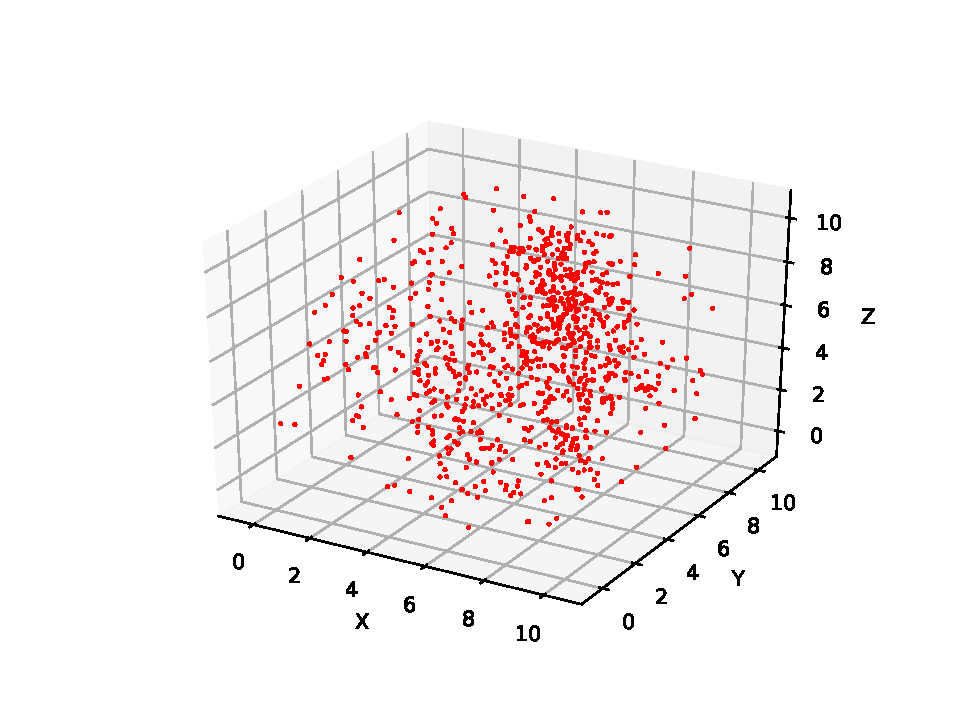
\includegraphics[width=4.5in]{galaxies.pdf}}
      \caption{3D plot of the galaxies in their initial locations at the start of the simulation.}
\end{figure}

\begin{figure}[!h]
	\centering
	\noindent
	\makebox[\textwidth]{
      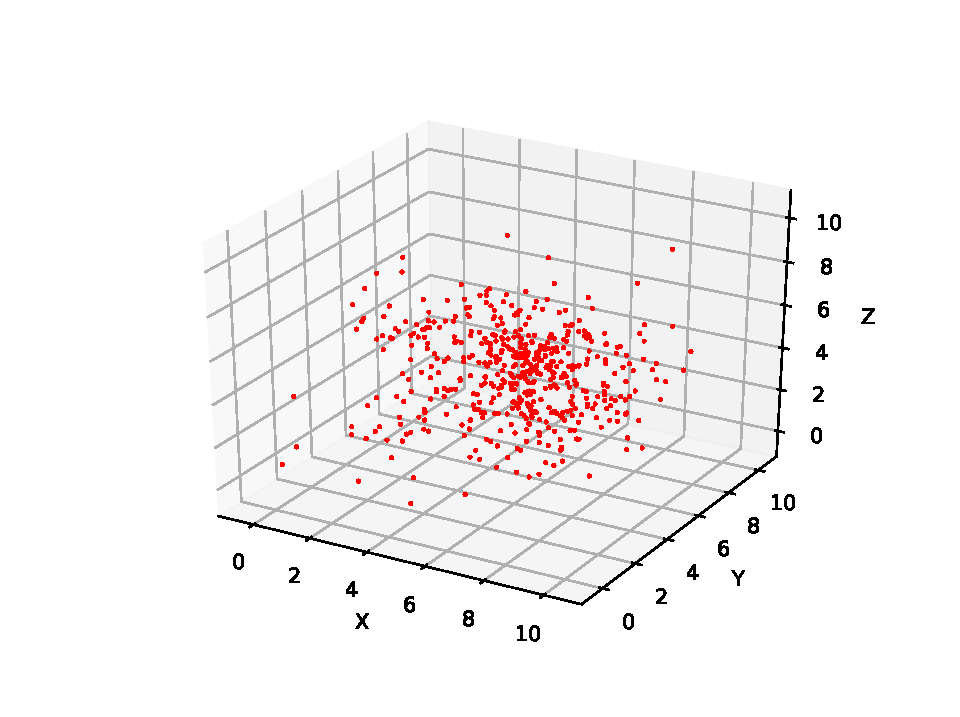
\includegraphics[width=4.5in]{finalplot.pdf}}
      \caption{3D plot of the galaxies at the end of the $10Gyr$ simulation.}
\end{figure}


\end{document}